\chapter{Specifikacija programske potpore}
		
	\section{Funkcionalni zahtjevi}
			
			
			\noindent \textbf{Dionici:}
			\begin{packed_enum}
				\item Neregistrirani korisnici
				\item Registrirani korisnici
					\begin{packed_enum}
						\item Izdavači
						\item Antikvarijati
						\item Preprodavači
					\end{packed_enum}
				\item Administratori
				\item Baza podataka
			\end{packed_enum}
			
			\noindent \textbf{Aktori i njihovi funkcionalni zahtjevi:}
			\begin{packed_enum}
			
				\item  \underbar{Neregistrirani korisnik (inicijator) može:}
				\begin{packed_enum}
					\item pretraživati ponudu knjiga po:
					\begin{packed_enum}
						\item  značajkama knjige 
						\item  ponuditelju
					\end{packed_enum}
					\item  pretraživati ponuditelje na karti
					\item odabrati ponuditelja i izlistati sve knjige u njegovoj ponudi
					\item zahtjevati od izdavača da kontaktira stranog izdavača za prijevod
					\item registrirati se 
						\begin{packed_item}
							\item unijeti podatke
						\end{packed_item}
				\end{packed_enum}
			
				\item  \underbar{Izdavač (inicijator) može:}
				\begin{packed_enum}
					\item zatražiti od stranog izdavača dozvolu za prijevod
					\item ponuditi knjige na hrvatskom jeziku
					\item maknuti knjige iz svoje ponude
				\end{packed_enum}
				
				\item  \underbar{Antikvarijat (inicijator) može:}
				\begin{packed_enum}
					\item ponuditi knjige na hrvatskom i srodnim jezicima
					\item maknuti knjige iz svoje ponude
				\end{packed_enum}
				
				\item  \underbar{Preprodavač (inicijator) može:}
				\begin{packed_enum}
					\item ponuditi knjige na bilo kojem jeziku
					\item maknuti knjige iz svoje ponude
				\end{packed_enum}
								
				\item \underbar{Administrator (inicijator) može:}
					\begin{packed_enum}
						\item odobriti registraciju
							\begin{packed_item}
								\item provjeriti je li adresa antikvarijata u RH i 
								\item jesu li ostali podatci dobri
							\end{packed_item}
						\item ukloniti registrirane korisnike
						\item mijenjati vrstu korisnika
						\item pristupiti bazi podataka
					\end{packed_enum}
					
				\item \underbar{Baza podataka (sudionik) pohranjuje podatke o:}
					\begin{packed_enum}
						\item registriranim korisnicima
						\item knjigama (uključujući i oznake knjige)
						\item zahtjevima za prijevod
					\end{packed_enum}
					
			\end{packed_enum}
			
			\eject 
			
			
				
			\subsection{Obrasci uporabe}
			
					\noindent \textbf{Opis obrazaca uporabe} \\
					

					\noindent \underbar{\textbf{UC1 - Pretraživanje knjiga po značajkama}}
					\begin{packed_item}
						\item \textbf{Glavni sudionik: }Neregistrirani korisnik
						\item  \textbf{Cilj:} Pregledati ponudu knjiga
						\item  \textbf{Sudionici:} Baza podataka
						\item  \textbf{Preduvjet:} -
						\item  \textbf{Opis osnovnog tijeka:}
						\item[] \begin{packed_enum}
							\item odabir značajki knjige po kojima se želi pretražiti
							\item prikazuje se ponuda knjiga s odabranim značajkama
						\end{packed_enum}
					\end{packed_item}
					
					\noindent \underbar{\textbf{UC2 - Pretraživanje knjiga po ponuditelju}}
					\begin{packed_item}
						\item \textbf{Glavni sudionik: }Neregistrirani korisnik
						\item  \textbf{Cilj:} Pregledati ponudu knjiga
						\item  \textbf{Sudionici:} Baza podataka
						\item  \textbf{Preduvjet:} -
						\item  \textbf{Opis osnovnog tijeka:}
						\item[] \begin{packed_enum}
							\item odabir ponuditelja čiju ponudu želi pregledati
							\item prikazuje se ponuda knjiga odabranog poslužitelja
						\end{packed_enum}
					\end{packed_item}
					
					\noindent \underbar{\textbf{UC3 - Pretraživanje ponuditelja na karti}}
					\begin{packed_item}
						\item \textbf{Glavni sudionik: }Neregistrirani korisnik
						\item  \textbf{Cilj:} Pregledati ponuditelje u blizini
						\item  \textbf{Sudionici:} Baza podataka
						\item  \textbf{Preduvjet:} -
						\item  \textbf{Opis osnovnog tijeka:}
						\item[] \begin{packed_enum}
							\item otvaranje karte s označenim ponuditeljima
							\item odabir lokacije i ponuditelja
							\item ispis podataka o ponuditelju i njihove ponude
						\end{packed_enum}
					\end{packed_item}
					
					\noindent \underbar{\textbf{UC4 - Zahtjev za prijevodom}}
					\begin{packed_item}
						\item \textbf{Glavni sudionik: }Neregistrirani korisnik
						\item  \textbf{Cilj:} Zatražiti prijevod knjige na stranom jeziku
						\item  \textbf{Sudionici:} Izdavač, baza podataka
						\item  \textbf{Preduvjet:} Knjiga nije prevedena na hrvatski
						\item  \textbf{Opis osnovnog tijeka:}
						\item[] \begin{packed_enum}
							\item odabir ~"Zahtjevaj prijevod" u sučelju aplikacije
							\item zahtjev se bilježi u bazu podataka
							\item izdavač dobija poruku o novom zahtjevu
						\end{packed_enum}
					\end{packed_item}
					
					\noindent \underbar{\textbf{UC5 - Registracija}}
					\begin{packed_item}
						\item \textbf{Glavni sudionik: }Neregistrirani korisnik
						\item  \textbf{Cilj:} Registrirati se kao ponuditelj
						\item  \textbf{Sudionici:} Baza podataka, administrator
						\item  \textbf{Preduvjet:} -
						\item  \textbf{Opis osnovnog tijeka:}
						\item[] \begin{packed_enum}
							\item odabir "Sign up" u sučelju
							\item unos vrste ponuditelja (izdavač, antikvarijat, preprodavač)
							\item unos podataka (naziv, e-pošta, adresa, broj telefona)
							\item unos korisničkog imena i lozinke
							\item administrator odobrava račun
							\item poruka na e-pošti o odobrenju ili neodobrenju računa
						\end{packed_enum}
						\item  \textbf{Opis mogućih odstupanja:}
						\item[] \begin{packed_item}
							\item[3.a] adresa antikvarijata nije u RH
							\item[] \begin{packed_enum}
								\item nemogućnost nastavka registracije bez promjene podataka
								\item upozorenje
							\end{packed_enum}
							\item[3.b] adresa preprodavača nije u zemlji srodnog jezika
							\item[] \begin{packed_enum}
								\item nemogućnost nastavka registracije bez promjene podataka
								\item upozorenje
							\end{packed_enum}
							\item[4.a] korisničko ime već postoji
							\item[] \begin{packed_enum}
								\item nemogućnost nastavka registracije bez promjene podataka
								\item upozorenje
							\end{packed_enum}	
						\end{packed_item}
					\end{packed_item}
					
					\noindent \underbar{\textbf{UC6 - Ponuda naslova knjiga}}
					\begin{packed_item}
						\item \textbf{Glavni sudionik: }Ponuditelj
						\item  \textbf{Cilj:} Ponuditi neograničen broj naslova knjiga
						\item  \textbf{Sudionici:} Baza podataka
						\item  \textbf{Preduvjet:} Registrirati se kao ponuditelj
						\item  \textbf{Opis osnovnog tijeka:}
						\item[] \begin{packed_enum}
							\item Ponuditelj odabire ~"Ponudi naslov knjige" u sučelju aplikacije
							\item Ponuditelj odabire naslove koje želi ponuditi
							\item U bazu podataka se pohrani promjena
						\end{packed_enum}
					\end{packed_item}
					
					\noindent \underbar{\textbf{UC7 - Ponuda primjeraka knjiga}}
					\begin{packed_item}
						\item \textbf{Glavni sudionik: }Ponuditelj
						\item  \textbf{Cilj:} Ponuditi neograničen broj primjeraka knjiga
						\item  \textbf{Sudionici:} Baza podataka
						\item  \textbf{Preduvjet:} Registrirati se kao ponuditelj
						\item  \textbf{Opis osnovnog tijeka:}
						\item[] \begin{packed_enum}
							\item Ponuditelj odabire ~"Ponudi primjerak knjige" u sučelju aplikacije
							\item Ponuditelj odabire primjerke knjiga
							\item U bazu podataka se pohrani promjena
						\end{packed_enum}
					\end{packed_item}
					
					\noindent \underbar{\textbf{UC8 - Pregled želja neregistriranih korisnika}}
					\begin{packed_item}
						\item \textbf{Glavni sudionik: }Izdavač
						\item  \textbf{Cilj:} Prikupiti želje neregistriranih korisnika
						\item  \textbf{Sudionici:} Baza podataka
						\item  \textbf{Preduvjet:} Registrirati se kao izdavač
						\item  \textbf{Opis osnovnog tijeka:}
						\item[] \begin{packed_enum}
							\item Praćenje aktivnosti neregistriranog korisnika
							\item Bilježenje i prikupljanje njegovih želja
						\end{packed_enum}
					\end{packed_item}
					
					\noindent \underbar{\textbf{UC9 - Zahtjev za dozvolu prijevoda sa stranog jezika}}
					\begin{packed_item}
						\item \textbf{Glavni sudionik: }Izdavač
						\item  \textbf{Cilj:} Zatražiti prijevod knjige sa stranog jezika na hrvatski
						\item  \textbf{Sudionici:} Baza podataka
						\item  \textbf{Preduvjet:} Registrirati se kao izdavač
						\item  \textbf{Opis osnovnog tijeka:}
						\item[] \begin{packed_enum}
							\item Izdavač pregleda želje neregistriranih korisnika
							\item Izdavač odabire knjige
							\item Izdavač zatraži dozvolu za prijevodom
						\end{packed_enum}
					\end{packed_item}
					
					\noindent \underbar{\textbf{UC10 - Zahtjev za dozvolu prijevoda sa srodnog jezika}}
					\begin{packed_item}
						\item \textbf{Glavni sudionik: }Izdavač
						\item  \textbf{Cilj:} Zatražiti prijevod knjige sa srodnog jezika na hrvatski
						\item  \textbf{Sudionici:} Baza podataka
						\item  \textbf{Preduvjet:} Registrirati se kao izdavač
						\item  \textbf{Opis osnovnog tijeka:}
						\item[] \begin{packed_enum}
							\item Izdavač pregleda želje neregistriranih korisnika
							\item Izdavač odabire knjige
							\item Izdavač zatraži dozvolu za prijevodom
						\end{packed_enum}
					\end{packed_item}
					
					\noindent \underbar{\textbf{UC11 - Ponuda knjiga na hrvatskom jeziku od strane izdavača}}
					\begin{packed_item}
						\item \textbf{Glavni sudionik: }Izdavač
						\item  \textbf{Cilj:} Ponuditi knjigu na hrvatskom jeziku
						\item  \textbf{Sudionici:} Baza podataka
						\item  \textbf{Preduvjet:}
						\item[] \begin{packed_enum}
							\item Registrirati se kao izdavač
							\item Imati u svojoj ponudi knjige na hrvatskom jeziku
						\end{packed_enum}
						\item  \textbf{Opis osnovnog tijeka:}
						\item[] \begin{packed_enum}
							\item Izdavač odabire knjige za ponudu
							\item Izdavač nudi odabrane knjige
							\item U bazu podataka se pohrani promjena
						\end{packed_enum}
					\end{packed_item}
					
					\noindent \underbar{\textbf{UC12 - Ponuda knjige na stranom jeziku od strane antikvarijata}}
					\begin{packed_item}
						\item \textbf{Glavni sudionik: }Antikvarijat
						\item  \textbf{Cilj:} Ponuditi knjige na stranom jeziku
						\item  \textbf{Sudionici:} Baza podataka
						\item  \textbf{Preduvjet:} Uspješna registracija kao antikvarijata
						\item  \textbf{Opis osnovnog tijeka:}
						\item[] \begin{packed_enum}
							\item Antikvarijat odabire knjige na stranom jeziku
							\item Antikvarijat nudi odabrane knjige
							\item U bazu podataka se pohrani promjena
						\end{packed_enum}
					\end{packed_item}
					
					\noindent \underbar{\textbf{UC13 - Ponuda knjige na srodnom jeziku od strane antikvarijata}}
					\begin{packed_item}
						\item \textbf{Glavni sudionik: }Antikvarijat
						\item  \textbf{Cilj:} Ponuditi knjige na srodnom jeziku
						\item  \textbf{Sudionici:} Baza podataka
						\item  \textbf{Preduvjet:} Uspješna registracija kao antikvarijata
						\item  \textbf{Opis osnovnog tijeka:}
						\item[] \begin{packed_enum}
							\item Antikvarijat odabire knjige na srodnom jeziku
							\item Antikvarijat nudi odabrane knjige
							\item U bazu podataka se pohrani promjena
						\end{packed_enum}
					\end{packed_item}
					
					\noindent \underbar{\textbf{UC14 - Ponuda knjige na hrvatskom jeziku od strane antikvarijata}}
					\begin{packed_item}
						\item \textbf{Glavni sudionik: }Antikvarijat
						\item  \textbf{Cilj:} Ponuditi knjige na hrvatskom jeziku
						\item  \textbf{Sudionici:} Baza podataka
						\item  \textbf{Preduvjet:} Uspješna registracija kao antikvarijata
						\item  \textbf{Opis osnovnog tijeka:}
						\item[] \begin{packed_enum}
							\item Antikvarijat odabire knjige na hrvatskom jeziku
							\item Antikvarijat nudi odabrane knjige
							\item U bazu podataka se pohrani promjena
						\end{packed_enum}
					\end{packed_item}
					
					\noindent \underbar{\textbf{UC15 - Ponuda knjige na stranom jeziku od strane preprodavača}}
					\begin{packed_item}
						\item \textbf{Glavni sudionik: }Preprodavač
						\item  \textbf{Cilj:} Ponuditi knjige na stranom jeziku
						\item  \textbf{Sudionici:} Baza podataka
						\item  \textbf{Preduvjet:} Uspješna registracija kao preprodavača
						\item  \textbf{Opis osnovnog tijeka:}
						\item[] \begin{packed_enum}
							\item Preprodavač odabire knjige na stranom jeziku
							\item Preprodavač nudi odabrane knjige
							\item U bazu podataka se pohrani promjena
						\end{packed_enum}
					\end{packed_item}
					
					\noindent \underbar{\textbf{UC16 - Ponuda knjige na srodnom jeziku od strane preprodavača}}
					\begin{packed_item}
						\item \textbf{Glavni sudionik: }Preprodavač
						\item  \textbf{Cilj:} Ponuditi knjige na srodnom jeziku
						\item  \textbf{Sudionici:} Baza podataka
						\item  \textbf{Preduvjet:} Uspješna registracija kao preprodavača
						\item  \textbf{Opis osnovnog tijeka:}
						\item[] \begin{packed_enum}
							\item Preprodavač odabire knjige na srodnom jeziku
							\item Preprodavač nudi odabrane knjige
							\item U bazu podataka se pohrani promjena
						\end{packed_enum}
					\end{packed_item}
					
					\noindent \underbar{\textbf{UC17 - Ponuda knjige na hrvatskom jeziku od strane preprodavača}}
					\begin{packed_item}
						\item \textbf{Glavni sudionik: }Preprodavač
						\item  \textbf{Cilj:} Ponuditi knjige na hrvatskom jeziku
						\item  \textbf{Sudionici:} Baza podataka
						\item  \textbf{Preduvjet:} Uspješna registracija kao preprodavača
						\item  \textbf{Opis osnovnog tijeka:}
						\item[] \begin{packed_enum}
							\item Preprodavač odabire knjige na hrvatskom jeziku
							\item Preprodavač nudi odabrane knjige
							\item U bazu podataka se pohrani promjena
						\end{packed_enum}
					\end{packed_item}
					
					\noindent \underbar{\textbf{UC18 - Određivanje ispravne oznake nove knjige}}
					\begin{packed_item}
						\item \textbf{Glavni sudionik: }Ponuditelj
						\item  \textbf{Cilj:} Ispravno odabrati oznaku vrste knjige kod dodavanja nove knjige
						\item  \textbf{Sudionici:} Baza podataka
						\item  \textbf{Preduvjet:} Registrirati se kao ponuditelj
						\item  \textbf{Opis osnovnog tijeka:}
						\item[] \begin{packed_enum}
							\item Ponuditelj odabire novu knjigu
							\item Ponuditelj odabire ispravnu vrstu oznake za tu knjigu
							\item U bazu podataka se pohrani promjena
						\end{packed_enum}
					\end{packed_item}
					
					\noindent \underbar{\textbf{UC19 - Određivanje ispravne oznake primjerka već dodane knjige}}
					\begin{packed_item}
						\item \textbf{Glavni sudionik: }Ponuditelj
						\item  \textbf{Cilj:} Ispravno odabrati oznaku vrste knjige za taj primjerak
						\item  \textbf{Sudionici:} Baza podataka
						\item  \textbf{Preduvjet:} Registrirati se kao ponuditelj
						\item  \textbf{Opis osnovnog tijeka:}
						\item[] \begin{packed_enum}
							\item Ponuditelj odabire već postojeću knjigu
							\item Ponuditelj odabire ispravnu vrstu oznake za tu knjigu
							\item U bazu podataka se pohrani promjena
						\end{packed_enum}
					\end{packed_item}
					
					
					\noindent \underbar{\textbf{UC20 - Ispravak oznake novog primjerka pri dodavanju}}
					\begin{packed_item}
						\item \textbf{Glavni sudionik: }Ponuditelj
						\item  \textbf{Cilj:} Izmijeniti pogrešno odabranu oznaku
						\item  \textbf{Sudionici:} Baza podataka
						\item  \textbf{Preduvjet:} Registrirati se kao ponuditelj
						\item  \textbf{Opis osnovnog tijeka:}
						\item[] \begin{packed_enum}
							\item Ponuditelj odabire primjerak s pogrešnom oznakom
							\item Ponuditelj ispravlja oznaku za taj primjerak knjige
							\item Ponuditelj dodaje primjerak knjige
							\item U bazu podataka se pohrani promjena
						\end{packed_enum}
					\end{packed_item}
					
					\noindent \underbar{\textbf{UC21 - Ispravak oznake novog primjerka pri uklanjanju}}
					\begin{packed_item}
						\item \textbf{Glavni sudionik: }Ponuditelj
						\item  \textbf{Cilj:} Izmijeniti pogrešno odabranu oznaku
						\item  \textbf{Sudionici:} Baza podataka
						\item  \textbf{Preduvjet:} Registrirati se kao ponuditelj
						\item  \textbf{Opis osnovnog tijeka:}
						\item[] \begin{packed_enum}
							\item Ponuditelj odabire primjerak s pogrešnom oznakom
							\item Ponuditelj ispravlja oznaku za taj primjerak knjige
							\item Ponuditelj uklanja primjerak knjige
							\item Iz baze podataka se uklanja primjerak knjige
						\end{packed_enum}
					\end{packed_item}
					
						\noindent \underbar{\textbf{UC22 - Odobravanje registracije}}
					\begin{packed_item}
						\item \textbf{Glavni sudionik: }Administrator
						\item  \textbf{Cilj:} Odobriti registraciju korisnika
						\item  \textbf{Sudionici:} Baza podataka
						\item  \textbf{Preduvjet:} Korisnik je registriran i dodijeljena su mu prava administratora
						\item  \textbf{Opis osnovnog tijeka:}
						\item[] \begin{packed_enum}
							\item Administrator pregleda zahtjev za registraciju
							\item Administrator provjerava odgovaraju li uneseni podaci
							\item Posebno za antikvarijata provjerava je li mu adresa u RH
							\item Ako je prijava ispravna, administrator odobrava registraciju korisnika
						\end{packed_enum}
					\end{packed_item}
					
					\noindent \underbar{\textbf{UC23 - Brisanje korisnika}}
					\begin{packed_item}
						\item \textbf{Glavni sudionik: }Administrator
						\item  \textbf{Cilj:} Izbrisati registriranog korisnika
						\item  \textbf{Sudionici:} Baza podataka
						\item  \textbf{Preduvjet:} Korisnik je registriran i dodijeljena su mu prava administratora
						\item  \textbf{Opis osnovnog tijeka:}
						\item[] \begin{packed_enum}
							\item Administrator odabire opciju uklanjanja korisnika
							\item Administrator pronalazi željenog korisnika
							\item Administrator uklanja željenog korisnika i njegove podatke iz baze podataka
						\end{packed_enum}
					\end{packed_item}
					
					\noindent \underbar{\textbf{UC24 - Promjena vrste korisnika}}
					\begin{packed_item}
						\item \textbf{Glavni sudionik: }Administrator
						\item  \textbf{Cilj:} Izmijeniti vrstu i prava korisnika
						\item  \textbf{Sudionici:} Baza podataka
						\item  \textbf{Preduvjet:} Korisnik je registriran i dodijeljena su mu prava administratora
						\item  \textbf{Opis osnovnog tijeka:}
						\item[] \begin{packed_enum}
							\item Administrator pronalazi željenog korisnika
							\item Administrator mijenja vrstu i prava korisnika \\
						\end{packed_enum}
					\end{packed_item}
					
					\eject 
				
					
				\subsubsection{Dijagrami obrazaca uporabe}
				
					\begin{figure}[H]
						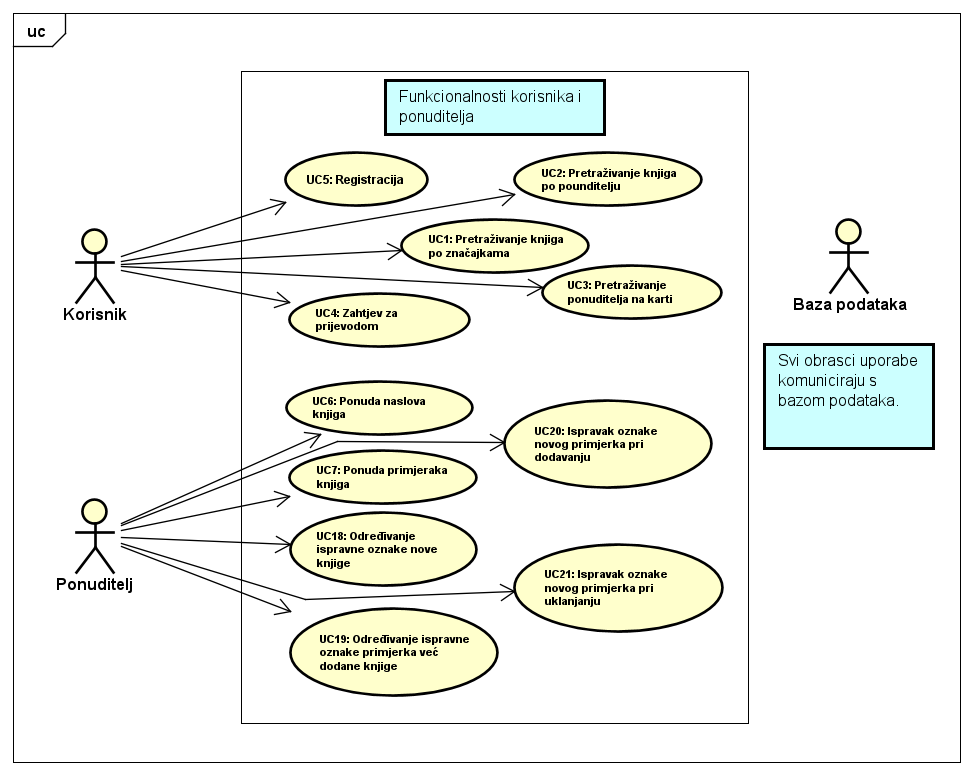
\includegraphics[width=\textwidth]{dijagrami/UseCaseD1.PNG} %veličina u odnosu na širinu linije
						\centering
						\caption{Dijagram obrasca uporabe, funkcionalnost korisnika i ponuditelja}
						\label{fig:promjene}
					\end{figure}
					
					\eject
					
					\begin{figure}[H]
						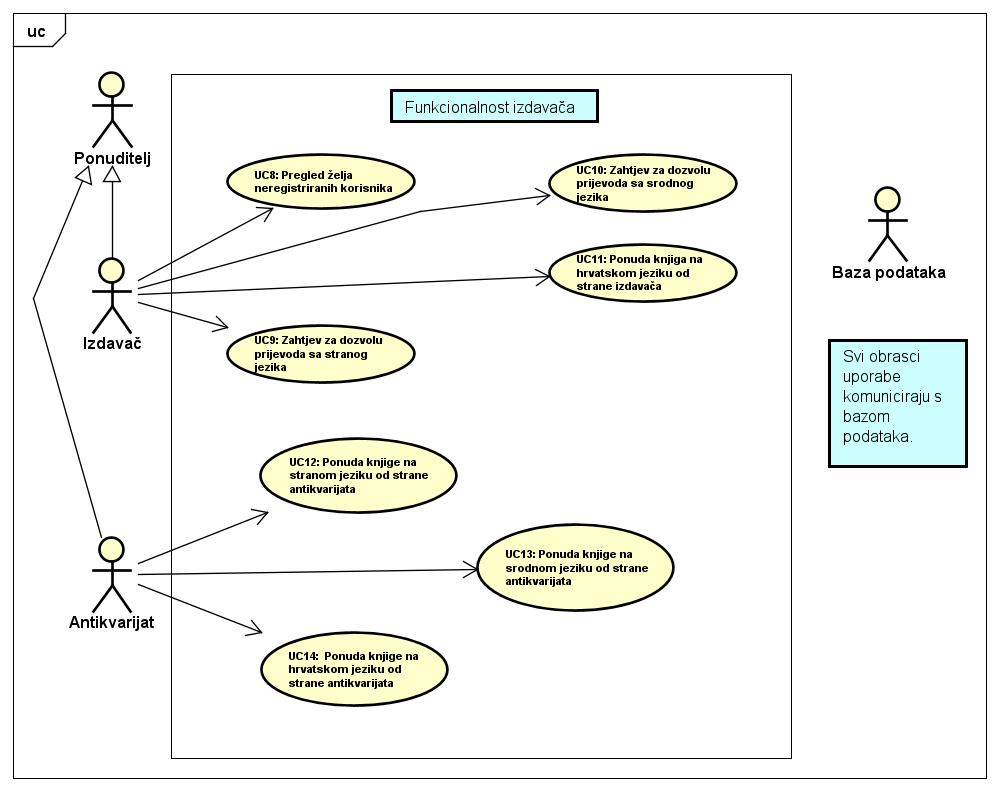
\includegraphics[width=\textwidth]{dijagrami/UseCaseD2.PNG} %veličina u odnosu na širinu linije
						\centering
						\caption{Dijagram obrasca uporabe, funkcionalnost izdavača i antikvarijata}
						\label{fig:promjene2}
					\end{figure}
					
					\eject
					
					\begin{figure}[H]
						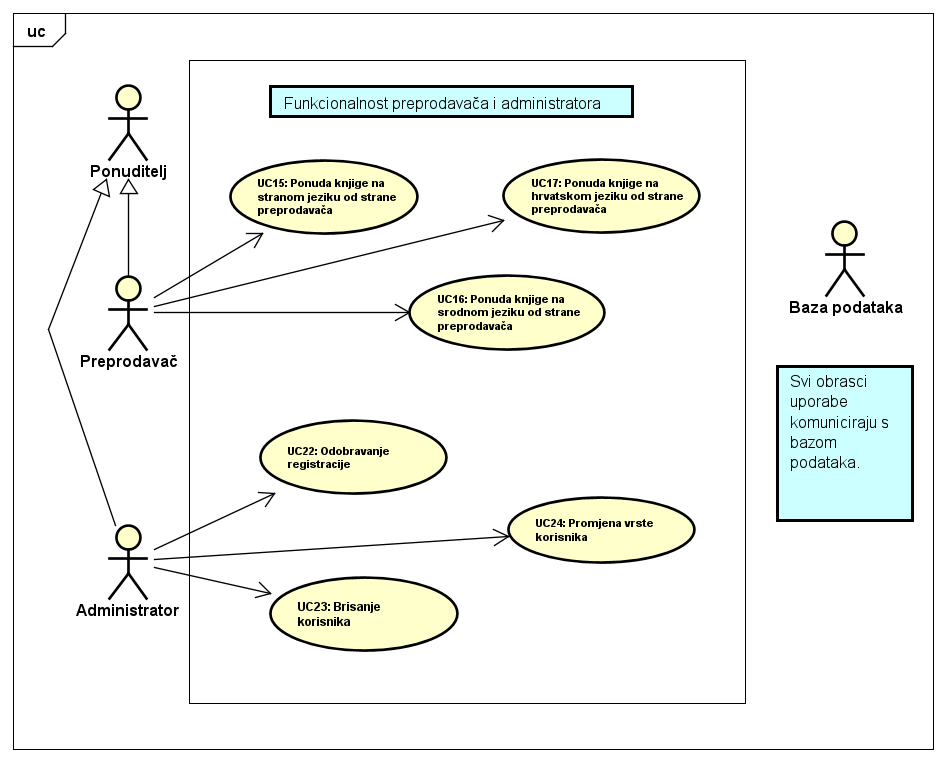
\includegraphics[width=\textwidth]{dijagrami/UseCaseD3.PNG} %veličina u odnosu na širinu linije
						\centering
						\caption{Dijagram obrasca uporabe, funkcionalnost preprodavača i administratora}
						\label{fig:promjene3}
					\end{figure}
					
					\eject
			
					
				
			\subsection{Sekvencijski dijagrami}
				
				\textbf{\textit{dio 1. revizije}}\\
				
				\textit{Nacrtati sekvencijske dijagrame koji modeliraju najvažnije dijelove sustava (max. 4 dijagrama). Ukoliko postoji nedoumica oko odabira, razjasniti s asistentom. Uz svaki dijagram napisati detaljni opis dijagrama.}
				\eject
	
		\section{Ostali zahtjevi}
		
			\textbf{\textit{dio 1. revizije}}\\
		 
			 \textit{Nefunkcionalni zahtjevi i zahtjevi domene primjene dopunjuju funkcionalne zahtjeve. Oni opisuju \textbf{kako se sustav treba ponašati} i koja \textbf{ograničenja} treba poštivati (performanse, korisničko iskustvo, pouzdanost, standardi kvalitete, sigurnost...). Primjeri takvih zahtjeva u Vašem projektu mogu biti: podržani jezici korisničkog sučelja, vrijeme odziva, najveći mogući podržani broj korisnika, podržane web/mobilne platforme, razina zaštite (protokoli komunikacije, kriptiranje...)... Svaki takav zahtjev potrebno je navesti u jednoj ili dvije rečenice.}
			 
			 
			 
	
